\subsubsection{Ingress}
\label{subsec:kubernetes:ingress}
Ingress dienen dem externen Zugriff auf die Dienste in einem Cluster \cite{kubernetesIngress}.
Hierbei werden HTTP und HTTPS Routen vom Cluster freigegeben, 
welche auf Service Objekte innerhalb des Cluster verweisen \cite{kubernetesIngress}.
Routen können basierend auf Pfaden oder Host-Headern an verschiedene Service Objekte und somit Pods verteilt werden \cite{kubernetesIngress}.
Dargestellt wird dieser Kommunikationsfluss in \ref{fig:ingress_communication}.

\begin{figure}[h]
  \centering
  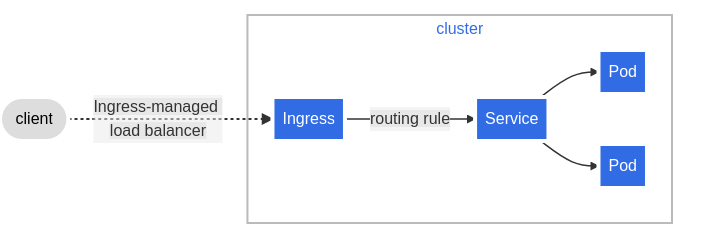
\includegraphics[width=\textwidth]{gfx/chapters/2_grundlagen/ingress.png}
  \caption{Ingress Kommunikation im Cluster}
  \label{fig:ingress_communication}
  \source{\cite{kubernetesIngress}}
\end{figure}

Kubernetes selbst definiert keinen Standard Controller, zum Verwalten von Ingress Objekten \cite{Burns2019}.
Nutzer müssen selbst dafür sorgen, einen Ingress Controller, 
wie beispielsweise den Nginx Ingress Controller \ref{sec:komponenten:externe-apps}, zu installieren \cite{Burns2019}.

Zur Verschlüsselung der Kommunikation können Ingress Objekten eine TLS Konfiguration übergeben werden.
Hierfür werden SSL Zertifikate sowie Schlüssel in Secret \ref{subsec:kubernetes:secret} Objekten gespeichert und im
Ingress Objekt referenziert. 
Zur Vereinfachung der Verwaltung dieser Zertifikate können Open Source Projekte wie \emph{Cert-Manager} \ref{sec:komponenten:externe-apps}
genutzt werden, welche die Verwaltung übernehmen \cite{Burns2019}.